%#BIBTEX bibtex Si$_3$N$_4$
\documentclass[twocolumn,amsmath,amssymb,a4paper,prb,superscriptaddress,floatfix]{revtex4-1}
\usepackage[dvipdfmx]{graphicx}
\usepackage{natbib}
\usepackage{multirow}
\usepackage{amsmath}
\usepackage{bm}
\usepackage{mathrsfs}
\usepackage{url}
\usepackage{color}
\usepackage{ulem}
\begin{document}

\title{First-principles calculation of lattice thermal
conductivities of $\alpha$-, $\beta$-, and $\gamma$-Si$_3$N$_4$}

\author{Kazuyoshi Tatsumi} \email{k-tatsumi@imass.nagoya-u.ac.jp}
\affiliation{Institute of
Materials and Systems for Sustainability, Nagoya University, Chikusa,
Nagoya 464-8603, Japan}
\affiliation{Center for Elements Strategy
Initiative for Structural Materials, Kyoto University, Sakyo, Kyoto
606-8501, Japan}

\author{Atsushi Togo}
\affiliation{Center for Elements Strategy Initiative for Structural
Materials, Kyoto University, Sakyo, Kyoto 606-8501, Japan}

\author{Isao Tanaka}
\affiliation{Center for Elements Strategy Initiative for Structural
Materials, Kyoto University, Sakyo, Kyoto 606-8501, Japan}
\affiliation{Department of Materials Science and
Engineering, Kyoto University, Sakyo, Kyoto 606-8501, Japan}
\affiliation{Nanostructures Research Laboratory, Japan Fine Ceramics
Center, Atsuta, Nagoya 456-8587, Japan}

\begin{abstract}
Lattice thermal conductivities of $\alpha$-, $\beta$- and $\gamma$-Si$_3$N$_4$
phases are investigated from {\it ab-initio} anharmonic lattice dynamics, within
the single-mode relaxation-time approximation of the linearized phonon Boltzmann
transport equation. At 300 K, the lattice thermal conductivity of
$\beta$-Si$_3$N$_4$ is calculated as $\kappa_{xx}=73$ and $\kappa_{zz}=198$ (in
units of Wm$^{-1}$K$^{-1}$), that is consistent with the reported experimental
values of 69 and 180, respectively. For $\alpha$-Si$_3$N$_4$, $\kappa_{xx}=69$
and $\kappa_{zz}=99$ are obtained.  The difference of anisotropy between these
phases is originated from their characteristic difference in the phonon band
structures, closely related to the crystal structures, specifically, the
stacking manners of equivalent basal layer structures.  In $\alpha$-Si$_3$N$_4$,
acoustic-mode phonons below 6 THz are the main heat carriers. In
$\beta$-Si$_3$N$_4$, the phonon modes up to 12 THz contribute to the lattice
thermal conductivity. In $\gamma$-Si$_3$N$_4$, $\kappa=81$ is obtained. The
distribution of phonon mode contributions to lattice thermal conductivity with
respect to phonon frequency is found to closely resemble that for $\kappa_{xx}$
of $\beta$-Si$_3$N$_4$ although the phonon lifetimes of $\gamma$-Si$_3$N$_4$ are
twice shorter than those of $\beta$-Si$_3$N$_4$.
\end{abstract}

\maketitle

\section{Introduction}
Several nitride insulators are known to exhibit high thermal conductivities and
are important for heat transfer materials at elevated temperatures. For example,
Slack {\it et al.}~\cite{slack} reported that wurtzite-type AlN has thermal
conductivity exceeding 100 Wm$^{-1}$K$^{-1}$. Si$_3$N$_4$ has become another
promising thermal conductive insulator because its thermal conductivity has been
improved up to 177 Wm$^{-1}$K$^{-1}$ by using the advanced ceramic technologies
related to the densification and microstructure
control.~\cite{zhou,hirao-rev,watari,hirosaki} Since the Si$_3$N$_4$ ceramics
also exhibit high mechanical strength at elevated temperatures, they are
regarded as ideal materials for the use in various applications, such as engine
components, gas turbines, and heat sink substrates of power semiconductor
devices.

At atmospheric pressure, Si$_3$N$_4$ has two phases, $\alpha$ and
$\beta$, which are generally considered as low- and high-temperature phases,
respectively.~\cite{zhou,hirosaki,riley} Their crystal structures belong to the
space groups of P31c and P6$_3$/m, respectively.~\cite{yashima,boulay} These
structures have different stacking manners of equivalent basal layer structures
composed of SiN$_4$ tetrahedra.~\cite{hampshire} In Fig.\ref{fig:Fig1_cryst}
these layer structures are depicted from the principal direction. They are
denoted as A, B, C, and D in the $\alpha$ phase and A and B in the $\beta$
phase, respectively. The stacking manners in $\alpha$- and $\beta$-Si$_3$N$_4$
are thus as ABCDABCD.. and ABAB.., respectively.  The $\alpha$ phase has
additional two layer structures of C and D, which are related to A and B by
the $c$ glide operation.~\cite{hampshire} Along this direction the lattice
constant of the $\alpha$ phase is approximately twice longer than that of the
$\beta$ phase.
\begin{figure}[ht]
 \begin{center}
  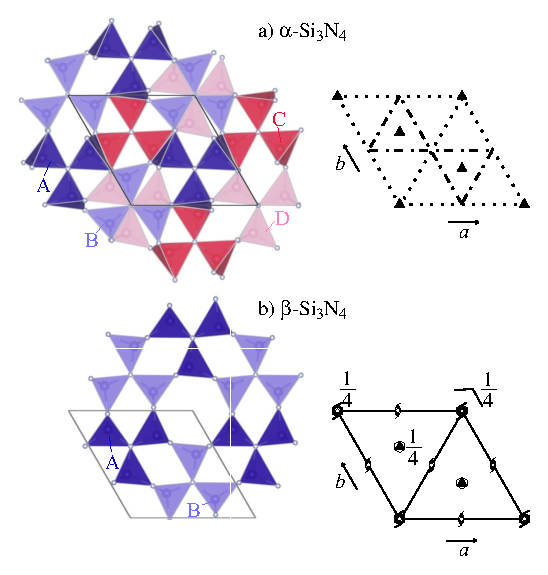
\includegraphics[width=0.90\linewidth]{Fig1_crystal_str2.eps} \caption{(color
  online) Crystal structures of $\alpha$- and $\beta$-Si$_3$N$_4$. Stacking of
  SiN$_4$ tetrahedron layers are shown in left. (a) ABCDABCD.. for
  $\alpha$-Si$_3$N$_4$. (b) ABAB.. for $\beta$-Si$_3$N$_4$.  Space group
  diagrams~\cite{inttableA} in P31c ($\alpha$-Si$_3$N$_4$) and P6$_3$/m ($\beta$-Si$_3$N$_4$)
  are shown in right.}
  \label{fig:Fig1_cryst} 
 \end{center}
\end{figure}

The experimental thermal conductivities
~\cite{zhou,hirao-rev,watari,hirosaki,hirai} of the Si$_3$N$_4$ polymorphs were
measured on the polycrystalline bulk samples. These values were significantly
affected by the lattice defects, impurities, shapes and orientations of the
constituent crystal grains;~\cite{hirosaki-md} the thermal conductivity
intrinsic to defect-free Si$_3$N$_4$ has not been established. As an
experimental approach for it, Li {\it et al.}~\cite{li} applied the
high-resolution thermoreflectance microscopy on single $\beta$-Si$_3$N$_4$
grains in a ceramic sample. Their analyzed thermal conductivity was 69 and 180
Wm$^{-1}$K$^{-1}$ along the $a$ and $c$ axes, respectively.  These values
respectively correspond to the $xx$ and $zz$ elements of the lattice thermal
conductivity tensor $\boldsymbol{\kappa}$. We consider the anisotropy of
$\kappa_{zz}/\kappa_{xx}\sim 3$ is relatively large.  Theoretically, Hirosaki
{\it et al.}~\cite{hirosaki-md} estimated the $\boldsymbol{\kappa}$ by applying
the Green-Kubo formulation to the molecular dynamics (MD) method with the
interatomic potentials proposed by Vashishta {\it et al.}~\cite{vashishta}.
They calculated $\kappa$$_{xx}$ and $\kappa$$_{zz}$ of $\alpha$-Si$_3$N$_4$ as
105 and 225 Wm$^{-1}$K$^{-1}$, and those of $\beta$-Si$_3$N$_4$ as 170 and 450
Wm$^{-1}$K$^{-1}$, respectively.  The ratio $\kappa_{zz}/\kappa_{xx}$ in
$\beta$-Si$_3$N$_4$ agreed well with the experimental ratio; the $\kappa_{xx}$
and $\kappa_{zz}$ overestimated the experimental $\boldsymbol{\kappa}$ more than
twice. 

Based on a first principles calculation and Boltzmann transport
theory~\cite{phono3py}, Togo {\it{et al.}} recently calculated
$\boldsymbol{\kappa}$ of many polymorphs of the zincblende- and wurtzite-type
structures. Their crystal structures have stacking orders of the densest atom
planes as ABCABC.. and ABAB.., respectively. The different stacking orders
merely altered the $\boldsymbol{\kappa}$.~\cite{phono3py} The phonon linewidths
and phonon density of states were merely altered as
well.~\cite{phono3py} On the other hand, the previous MD results on $\alpha$-
and $\beta$-Si$_3$N$_4$ presented that the different stacking orders in these
phases altered the $\boldsymbol{\kappa}$ largely. This has not been explained
through their phonon properties.  It is interesting to investigate it using the
first principles anharmonic phonon calculation.

In addition to the $\alpha$ and $\beta$ phases, a cubic spinel phase
($\gamma$-Si$_3$N$_4$) is known to form upon compression and in-situ
heating.~\cite{zerr,zhang} The reported transition pressures are scattered from
10 to 36 GPa depending on the experimental conditions.~\cite{xu}  The $\gamma$
phase is experimentally quenched to atmospheric pressure and room temperature.
Its thermal conductivity has not been experimentally reported; it has been
estimated by the Slack model.~\cite{morelli} 

The present study aims to qualitatively understand the lattice thermal
conductivity tensors among the three Si$_3$N$_4$ phases by means of the first
principles approach.  We calculate the $\boldsymbol{\kappa}$ of the $\gamma$
phase as well, for systematic understanding. After the methodology section, we
examine the validity of the present results first.  Our calculated thermal
properties are compared with the available experimental and theoretical
references.  Then we investigate the characteristic behaviors of the 
$\boldsymbol{\kappa}$ in detail on the basis of the phonon band structures and
phonon linewidths.

\section{Computational procedures}

\subsection{Lattice thermal conductivity calculation}

The lattice thermal conductivities were calculated by solving the linearized
Boltzmann transport equation (LBTE) within the single-mode relaxation time
approximation (single-mode RTA).  We also tried the direct-solution of
LBTE~\cite{chaput-direct} and leave its calculated $\boldsymbol{\kappa}$ values
in the following section. The differences between the
$\boldsymbol{\kappa}$ calculated by the single-mode RTA and the direct solution
were found minor for our discussion. Therefore we limited our research to use
the single-mode RTA to take advantage of its intuitive closed form of
$\boldsymbol{\kappa}$.

In the following sections, we denote a phonon mode by $\lambda=(\mathbf{q},p)$
with the set of the phonon wave vector $\mathbf{q}$ and band index $p$ and $-\lambda \equiv (-\mathbf{q},p)$. The
relaxation time due to phonon-phonon scattering was obtained as reciprocal of
linewidth, $\tau_{\lambda,\text{ph-ph}}=(2\Gamma_\lambda)^{-1}$, where the
linewidth that we employed in this study is as follows:
\begin{align}
 \label{eq:linewidth}
 &\Gamma_\lambda = \frac{18\pi}{\hbar^2}
  \sum_{\lambda' \lambda''}
  \bigl|\Phi_{-\lambda\lambda'\lambda''}\bigl|^2 \times \nonumber \\ 
 &\left\{ (n_{\lambda'} + n_{\lambda''}+1) 
   \delta(\omega_\lambda-\omega_{\lambda'}-\omega_{\lambda''}) \right.
   + \nonumber \\ 
 &\;\;(n_{\lambda'}-n_{\lambda''})
  \left[\delta(\omega_\lambda +\omega_{\lambda'}-\omega_{\lambda''})
 \right. 
 \left. -\left. \delta(\omega_\lambda - \omega_{\lambda'}+\omega_{\lambda''})
 \right]\right\}.
\end{align}
Here $\omega_\lambda$ is the harmonic phonon frequency of the phonon mode
$\lambda$, $n_\lambda=[\exp(\hbar\omega_\lambda/\mathrm{k_B}T)-1]^{-1}$ is
the Bose-Einstein distribution at temperature $T$, and
$\Phi_{\lambda\lambda'\lambda''}$ denotes the three-phonon-scattering strength.
$\Phi_{\lambda\lambda'\lambda''}$ was obtained by usual coordinate
transformation of third-order force constants from direct space to phonon
space.~\cite{phono3py} The second- and third-order real-space force constants
were obtained from the {\it ab-initio} calculation, whose details are written in the
next section.

In order to compare the more realistic results of the calculated $\boldsymbol{\kappa}$ with the
experimental thermal conductivities, the isotopic scattering effect due to the natural isotope
distribution was taken into account according to the second-order perturbation
theory.~\cite{tamura} With the relaxation times of the phonon-phonon scattering
and isotopic scattering, $\tau_{\lambda,\text{ph-ph}}$ and
$\tau_{\lambda,\text{iso}}$, the total relaxation time for a phonon mode was
assumed to be $1/\tau_{\lambda} = 1/\tau_{\lambda,\text{ph-ph}} +
1/\tau_{\lambda,\text{iso}}$, according to Matthiessen's rule.

The available experimental thermal conductivities in the Si$_3$N$_4$ system were
measured on the polycrystalline samples and not measured from any single
crystals. The conductivities measured at a polycrystalline area were affected
by various lattice defects within it , such as grain boundaries, impurities, and
vacancies, we crudely took them into account by a relaxation time
$\tau_{\lambda,\text{bs}}=L/|\mathbf{v}_\lambda|$ of a phonon boundary
scattering model, where $\mathbf{v}_\lambda = \nabla_{\mathbf{q}}\omega_\lambda$
is the group velocity and $L$ a parameter regarding to the boundary mean free
path. We consider $\tau_{\lambda,\text{bs}}$ as a variable parameter and partly
include it to $\boldsymbol{\kappa}$ according to Matthiessen's rule. 

The closed form of $\boldsymbol{\kappa}$ within RTA was obtained via
\begin{align}
 \label{eq:kappa}
 \boldsymbol{\kappa}(T) = \frac{1}{N_\mathbf{q}\Omega} \sum_\lambda
 \tau_\lambda(T) \mathbf{v}_\lambda \otimes \mathbf{v}_\lambda c_\lambda(T),
\end{align}
where $N_\mathbf{q}$ is the number of
$\mathbf{q}$-points, $\Omega$ is the unit cell volume, and $c_\lambda$
is the mode heat capacity. To analyze $\boldsymbol{\kappa}$ in detail, we calculate
the cumulative thermal conductivity:
\begin{align}
 \label{eq:cum-kappa}
 \boldsymbol{\kappa}^\text{c}(\omega) = \frac{1}{N_\mathbf{q}\Omega}
 \int_0^\omega \sum_\lambda
 \tau_\lambda(T) \mathbf{v}_\lambda \otimes \mathbf{v}_\lambda
 c_\lambda(T) \delta(\omega'-\omega)d\omega',
\end{align}
and its derivative $\frac{\partial
\boldsymbol{\kappa}^\text{c}(\omega)}{\partial \omega}$ to see the phonon mode
contributions to $\boldsymbol{\kappa}$.

The lattice thermal conductivities were calculated with the phonon-phonon interaction calculation code
phono3py~\cite{phono3py}, while the harmonic phonon states were analyzed with
the phonon calculation code phonopy~\cite{phonopy}.

\subsection{Computational details}

The force constants were calculated using the first-principles projector
augmented wave method~\cite{paw} (VASP code~\cite{vasp-1996,vasp-1995,
vasp-1999}). The generalized gradient approximation (GGA) parameterized by
Perdew, Burke, and Ernzerhof~\cite{pbe} was used for the exchange correlation
potential. A plane wave energy cutoff of 500 eV was employed. The crystal
structures were optimized until the residual forces acting on the constituent
atoms were less than $10^{-6}$ eV/\AA. The structural optimization was firstly
performed for a temperature of 0 K and 0 GPa. Here the temperature and pressure
were considered only for the electronic system and the zero point lattice
vibration was not taken into account. The calculated lattice parameters were
$a=7.808$ \AA~ and $c=5.659$ \AA~ for the $\alpha$ phase, $a=7.660$ \AA~ and
$c=2.925$ \AA~ for the $\beta$ phase, and $a=7.787$ \AA~ for the $\gamma$ phase,
which agree with the experimental data~\cite{yashima,boulay,paszkowicz} within
+0.7 \% errors. The lattice volume optimized with the local density
approximation (LDA)~\cite{lda} for the exchange correlation potential was, for
$\beta$-Si$_3$N$_4$, 3 \% smaller than the volume with GGA, which is a typical
volume contraction of LDA. The $\boldsymbol{\kappa}$ calculated with LDA was
larger by 2.6 \% than the $\boldsymbol{\kappa}$ with GGA. For our discussion,
this difference is enough small, therefore the impact of choice of exchange
correlation potential is considered to be minor in our study.

\begin{table}[ht]
	\caption{\label{table:LTC} Calculated lattice thermal conductivities 
 of $\alpha$-, $\beta$-, and $\gamma$-Si$_3$N$_4$
 (WK$^{-1}$m$^{-1}$) at 300 K with respect to several combinations of
 supercell sizes.}
 \begin{ruledtabular}
  \begin{tabular}{ccccc}
   \multirow{2}{*}{Phase}
   & \multicolumn{2}{c}{Supercell (\# of atoms)} &
   \multicolumn{2}{c}{LTC} \\
   \cline{2-5}
   & $3^\text{rd}$ force constants & $2^\text{nd}$ force constants & $xx$ & $zz$ \\
   \hline
   \multirow{6}{*}{$\alpha$}
   & $1\times 1\times 1$ (28) & $1\times
   1\times 1$ (28) & 37 &   57 \\ 
   & $1\times 1\times 2$ (56) & $1\times
   1\times 2$ (56) & 41 &   79 \\ 
   & $1\times 1\times 1$ (28) & $2\times
   2\times 2$ (224) & 55 &   81 \\ 
   & $1\times 1\times 2$ (56) & $2\times
   2\times 2$ (224) & 67 &   95 \\ 
   & $1\times 1\times 2$ (56) & $2\times
   2\times 3$ (336) & 68 &  97 \\ 
   & $1\times 1\times 2$ (56) & $3\times
   3\times 4$ (1008) & 68 &  100 \\ 
   \hline
   \multirow{5}{*}{$\beta$}
   & $1\times 1\times 2$ (28) & $1\times
   1\times 2$ (28) & 44 & 173 \\ 
   & $1\times 1\times 2$ (28) & $2\times
   2\times 4$ (224) & 76 &  208 \\ 
   & $1\times 1\times 3$ (42) & $2\times
   2\times 4$ (224) & 71 & 194 \\ 
   & $1\times 1\times 3$ (42) & $2\times
   2\times 5$ (280) & 72 & 196 \\ 
   & $1\times 1\times 3$ (42) & $3\times
   3\times 8$ (1008) & 73 & 199 \\ 
   \hline
   \multirow{3}{*}{$\gamma$}
   & $1\times 1\times 1$ (56) & $1\times
   1\times 1$ (56) & \multicolumn{2}{c}{72} \\ 
   & $1\times 1\times 1$ (56) & $2\times
   2\times 2$ (448) & \multicolumn{2}{c}{77} \\ 
   & $1\times 1\times 1$ (56) & $3\times
   3\times 3$ (56) & \multicolumn{2}{c}{79} \\ 
  \end{tabular}
 \end{ruledtabular}
\end{table}

The force constants were calculated by the finite difference
approach~\cite{wei-supercell}. For this calulation, we adopted the following
supercells: The $1\times 1\times2$, $1\times 1\times3$, and $1\times 1\times1$
supercells of the conventional unit cells for the third-order force constants of
$\alpha$, $\beta$, and $\gamma$-Si$_3$N$_4$, respectively, and the $3\times
3\times4$, $3\times 3\times8$ and $2\times 2\times2$ for the second-order force
constants.  The length of the induced atomic displacements was set to 0.03 \AA.
Table \ref{table:LTC} shows the $\boldsymbol{\kappa}$  calculated with several
different sets of the supercells, indicating that our calculated
$\boldsymbol{\kappa}$ is reasonably converging with respect to the size of the
supercells. 

Uniform $\mathbf{k}$-point sampling meshes of $4\times 4\times 2$, $4\times
4\times 3$, and $3\times 3\times 3$ were used for the third-order force
constants of the $\alpha$, $\beta$, and $\gamma$ phases. For the $\alpha$ and
$\beta$ phases the center of the $a^*b^*$ plane was sampled while the center on
the $c^*$-axis was not. For the $\gamma$ phase, non-$\Gamma$ center mesh was
used. For the second-order force constants, the $\Gamma$-point was only sampled
for the $\alpha$ and $\beta$ phase and the only one $\mathbf{k}=(0.5, 0.5, 0.5)$
point was sampled for the $\gamma$ phase. The $\mathbf{q}$-point sampling meshes
of $10\times 10\times 14$, $10\times 10\times 26$, and $12\times 12\times 12$
were used to calculate $\boldsymbol{\kappa}$ in Eq.~(\ref{eq:kappa}) for the
$\alpha$, $\beta$, and $\gamma$ phases.

Non-analytical term correction~\cite{wang} was applied to the second-order force
constants to take into account the long range Coulomb forces present in ionic
crystals. For the correction, static dielectric constants and Born effective
charges were calculated by using the density functional perturbation theory
(DFPT) as implemented in the VASP code~\cite{vasp-lepsiron,lepsiron}.

We examined the effect of thermal expansion on $\boldsymbol{\kappa}$. For this,
we calculated the $\boldsymbol{\kappa}$ with the crystal structures which were
optimized for several finite temperatures within the quasi-harmonic
approximation (QHA)~\cite{dove-p76}. These $\boldsymbol{\kappa}$ were different
from the $\boldsymbol{\kappa}$ for the corresponding temperatures, calculated
with the structure which was initially optimized for 0 K. We consider these
differences as the effect of thermal expansion.  We calculated the differences
between the $\beta$-Si$_3$N$_4$ structures for $T$=300, 600, 900, 1200, and,
1500 K. The differences were found within 1 \%, similar to the case of Si and
Ge~\cite{ward-ltc}. For the present study, these differences are negligible and
we adopt the $\boldsymbol{\kappa}$ calculated with the structure which was
initially optimized for 0 K.


In addition, we calculated the volumetric thermal expansion coefficients. Their
comparison with the experimental coefficients is useful to validate the present
thermal conductivity calculation, because the thermal expansion is originated
from the anharmonicity of the interatomic potential as well as
$\boldsymbol{\kappa}$. The calculated coefficients of the $\alpha$ and $\beta$
phases were 4.31$\times 10^{-6}$ and 4.19$\times 10^{-6}$ K$^{-1}$ for 300 K,
while the experimental values~\cite{minikayev-alpha} are 3.75$\times 10^{-6}$
and 3.55$\times 10^{-6}$ K$^{-1}$. The calculation reproduced the
experimental tendency where the $\alpha$ phase has a slightly larger thermal
expansion coefficient than the $\beta$ phase. This supports that the present
calculation enables us to qualitatively compare the calculated
$\boldsymbol{\kappa}$ among the Si$_3$N$_4$ phases.

In order to compare the microscopic phonon properties among the three phases at
the same conditions, those results calculated at 0 GPa are shown and discussed.
For the $\gamma$ phase, this means that we assume the condition of a virtually
quenched $\gamma$ phase at 0 GPa from the high pressure. To examine the
analytical continuity of the properties with respect to pressures, we
calculated $\boldsymbol{\kappa}$ of the $\gamma$ phase at 10, 20, and 40 GPa as
shown in Fig.~\ref{fig:S1}. The phenomenological behaviour of linear dependence
of $\boldsymbol{\kappa}$ with respect to pressure was reproduced as similar to
Ref.~\onlinecite{andersson-pressure}. The slope was 2.89
Wm$^{-1}$K$^{-1}$GPa$^{-1}$ for the $\gamma$ phase.  By this dependence, we
consider that the microscopic values are also varied smoothly with the pressure
and those at 0 GPa are valuable to compare with the $\alpha$ and $\beta$
phases.

\subsection{Direct solution of LBTE}

The merit to employ the single-mode RTA for thermal conductivity calculation is
the closed form, by which we can intuitively understand the qualitative
character of $\boldsymbol{\kappa}$ in terms of the relaxation time and group
velocity. The microscopic understanding of the full solution of LBTE is still
under the development~\cite{cepellotti-relaxons} and the microscopic picture
based on collective phonons~\cite{hardy-collective} will require more
complicated investigation.

It is known that the single-mode RTA solution of LBTE often underestimates the
full solution.~\cite{mukhopadhyay-ltc,ward-ltc} To check the underestimation, we
calculated $\boldsymbol{\kappa}$ of the $\alpha$ and $\beta$ phases by a direct
solution of LBTE~\cite{chaput-direct}, which is one of the methods of LBTE full
solutions. Their $\kappa_{xx}$ and $\kappa_{zz}$ without the isotope effect were
69 and 102 Wm$^{-1}$K$^{-1}$ for  the $\alpha$ phase and 76 and 238
Wm$^{-1}$K$^{-1}$ for the $\beta$ phase, respectively, while the corresponding
single-mode RTA values were 70 and 102 Wm$^{-1}$K$^{-1}$ for the $\alpha$ phase
and 76 and 210 Wm$^{-1}$K$^{-1}$ for the $\beta$ phase. The $\kappa_{zz}$ of the
direct solution in the $\beta$ phase was 13 \% larger than that of the
single-mode RTA solution. Since the differences in $\boldsymbol{\kappa}$ between
the LBTE solutions are not significant, we expect the physics on those lattice
thermal conductivities is well understood within the single-mode RTA in the
current level of our interest. Therefore, we discuss the lattice thermal
conductivities calculated by the single-mode RTA solution.

\section{Results and discussion}

\subsection{Lattice thermal conductivities}

\begin{table}[ht]
 \caption{\label{table:LTC-exp} Calculated thermal conductivities of
 $\alpha$-Si$_3$N$_4$ (trigonal), $\beta$-Si$_3$N$_4$ (trigonal), and
 $\gamma$-Si$_3$N$_4$ (cubic) at 300
 K, compared with the experimental and theoretical reference data. Theoretical bulk moduli $B$ in
 units of GPa, calculated by the authors by using the present band
 method, are additionarily presented in the fourth column.}

\begin{ruledtabular}
 \begin{tabular}{ccccccccc}
   & \multicolumn{3}{c}{This work} & \multicolumn{3}{c}{Ref. Theo.}
   & \multicolumn{2}{c}{Ref. Expt.} \\
   \cline{2-9}
   & $\kappa_{xx}$ & $\kappa_{zz}$ & $B$ & $\kappa$ & $\kappa_{xx}$ & $\kappa_{zz}$ & $\kappa_{xx}$ & $\kappa_{zz}$ \\
   \hline
   $\alpha$-Si$_3$N$_4$ & 68 & 100 & 224 & 70\footnotemark[1] & 105\footnotemark[2] & 225\footnotemark[2] & - & -  \\
   $\beta$-Si$_3$N$_4$ & 73 & 199 & 237 & 250\footnotemark[1] & 170\footnotemark[2] & 450\footnotemark[2] & 69\footnotemark[3] & 180\footnotemark[3] \\
   $\gamma$-Si$_3$N$_4$ & 77 & - & 296 & 80\footnotemark[1] & - & - & - & - 
   \footnotetext[1]{Ref.~\onlinecite{morelli}, Slack model.}
   \footnotetext[2]{Ref.~\onlinecite{hirosaki-md}, molecular dynamics (Green-Kubo).}
   \footnotetext[3]{Ref.~\onlinecite{li}, single crystalline grains of poly-crystals.}
  \end{tabular}
 \end{ruledtabular}
\end{table}

Table \ref{table:LTC-exp} shows the present results of the
$\boldsymbol{\kappa}$ for 300 K.  $\beta$-Si$_3$N$_4$ has a markedly more
anisotropic $\boldsymbol{\kappa}$ than $\alpha$-Si$_3$N$_4$.  The directional
averages $\sum_i \kappa_{ii}/3$  are 79, 115,  and 77 Wm$^{-1}$K$^{-1}$ for the
$\alpha$, $\beta$, and $\gamma$ phases, respectively.  The value of the
$\gamma$ phase is similar to that of the $\alpha$ phase, in spite of
comparatively large difference among the bulk moduli ($B$) that are also shown
in Table \ref{table:LTC-exp}.   

Table \ref{table:LTC-exp} also lists the previously reported
experimental~\cite{li} and theoretical~\cite{hirosaki-md} $\boldsymbol{\kappa}$
for the references.  The theoretical results~\cite{morelli} of the Slack model,
which do not include the anisotropy in $\boldsymbol{\kappa}$, are shown as
$\kappa$ in Table \ref{table:LTC-exp}.  For the $\beta$ phase, compared to the
$\boldsymbol{\kappa}$ of the molecular dynamics~\cite{hirosaki-md}, our
$\boldsymbol{\kappa}$ agrees better with the experimental $\boldsymbol{\kappa}$.
Also, compared to the $\kappa$ of the Slack model, our directional average
$\sum_i \kappa_{ii}/3$ is much closer to the experimental average. 

Fig.~\ref{fig:Fig1_338} shows the theoretical $\boldsymbol{\kappa}$ of the
$\alpha$ and $\beta$ phases as a function of $T$, together with the reference
experimental data~\cite{hirosaki,hirai}. The experimental thermal conductivities
for a series of temperatures were measured on the polycrystalline sample areas
by the laser flash method. These thermal conductivities (denoted as
$\kappa_\mathrm{polycrystal}$) cannot be directly compared with the calculated
intrinsic $\boldsymbol{\kappa}$ because they largely depended on the
microstructure of the samples: They were deviated from the simple directional
averages of the intrinsic $\kappa_{ii}$, depending on the shapes of the crystal
grains.  We treated this effect by using a parameter $0\le{w}\le{1}$ and fitting
the quantities of $w\kappa_{xx} + (1-w) \kappa_{zz}$ to the experimental
$\kappa_\mathrm{polycrystal}$ by the least squares method. We consider these as
theoretical $\kappa_\mathrm{polycrystal}$. 

\begin{figure}[ht]
 \begin{center}
  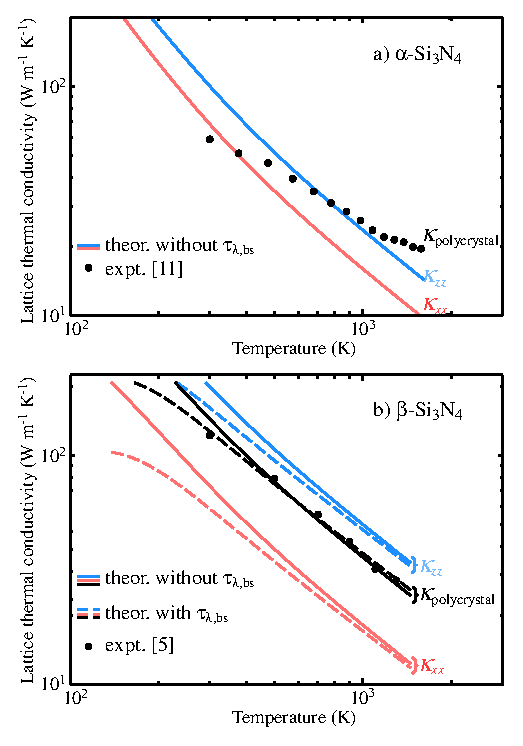
\includegraphics[width=0.90\linewidth]{Fig1_m1010.eps} \caption{(color
  online) Temperature dependences of thermal conductivities for $\alpha$- and
  $\beta$-Si$_3$N$_4$. For $\beta$-Si$_3$N$_4$, theoretical conductivities with the
  boundary scattering effect are shown by broken lines. Theoretical
  $\kappa_\mathrm{polycrystal}$ 
  (see in text) for the $\beta$-Si$_3$N$_4$ sample are
  also shown to be compared with the experimental conductivities.}
  \label{fig:Fig1_338}
 \end{center}
\end{figure}

In Fig.~\ref{fig:Fig1_338}, the $\kappa_{ii}$ calculated without
$\tau_{\lambda,\text{bs}}$ are nearly proportional to $T^{-1}$ because
$n_\lambda$ in Eq.~(\ref{eq:linewidth}) can be reduced to
$\exp(-\hbar\omega_\lambda/\mathrm{k_B}T)$. In Fig.~\ref{fig:Fig1_338}-a, the
experimental $\kappa_\mathrm{polycrystal}$ of a chemically vapor-deposited
$\alpha$-Si$_3$N$_4$ sample~\cite{hirai} is not proportional to $T^{-1}$ and
intersects the theoretical $\kappa_{ii}$.  Thus no value of $w$ adjusts the
theoretical $\kappa_\rm{polycrystal}$ to the experimental
$\kappa_\rm{polycrystal}$.  The full solution of LBTE
would negligibly cure the disagreement.  Including the simple phonon lifetime of
boundary scattering, $\tau_{\lambda,\text{bs}}=L/|\mathbf{v}_\lambda|$, into the
total phonon lifetime according to Matthiessen's rule, could not explain the
discrepancy as well. A $L$ value of 0.6 $\mu\text{m}$, which was much smaller
than the experimental grain size~\cite{hirai} of 10 $\mu\text{m}$, decreased the
theoretical $\kappa$$_{ii}$ in the low temperature side toward the experimental
values, but kept the $\kappa$$_{ii}$ in the high temperature side severely
smaller than the experimental values. At present, the reason for the discrepancy
between the theoretical and experimental behaviors is unclear.  Although the
crystal structure of the experimental sample was characterized as
$\alpha$-Si$_3$N$_4$, significant lattice defects existed in the sample as
pointed out by Hirosaki {\it et al.}~\cite{hirosaki-md} and the simple phonon
boundary scattering model may fail to describe their effects on the
$\kappa_\mathrm{polycrystal}$. 

For the $\beta$ phase, the experimental $\kappa_\mathrm{polycrystal}$ are located
in-between the theoretical $\kappa$$_{xx}$ and  $\kappa$$_{zz}$, being nearly
proportional to $T^{-1}$. Simple directional averages of the theoretical
$\kappa_{ii}$ slightly underestimate these experimental values.  This is
understood from the fact that the microstructure was controlled to increase the
$\kappa_\mathrm{polycrystal}$, and the crystalline grains were selectively grown
along the $c$ axis of the most conductive direction.~\cite{hirosaki} The
theoretical $\kappa_\mathrm{polycrystal}$ were fit well with $w=0.44$  to the
experimental.  For the effects of lattice defects most of which were grain
boundaries, we included $\tau_{\lambda,\text{bs}}$ with $L=0.6$ $\mu\text{m}$ to
further fit the theoretical curve ($w=0.33$) to the experimental data.  The $L$
value is slightly smaller than the average grain size~\cite{hirosaki} of 2
$\mu\text{m}$ in the experiment.


\subsection{Dispersion curves}

\begin{figure}[ht]
 \begin{center}
  \includegraphics[width=0.90\linewidth]{Fig4_ver5_338_resize2_woDOS.eps}
  \caption{(color online) Brillouin-zones (left) and calculated phonon band diagrams (right) for three Si$_3$N$_4$ phases.
  \label{fig:Fig4_ver5_338} }
 \end{center}
\end{figure}

Figure \ref{fig:Fig4_ver5_338} shows the phonon band diagrams of the three
Si$_3$N$_4$ phases. The entire band diagrams are almost identical to those
reported earlier~\cite{kuwabara,xu}. However, here we investigate the gradients
within the band dispersions, that is, the group velocities projected on the
high-symmetry paths. We especially focus on their anisotropy in the $\alpha$ and
$\beta$ phases. This was not investigated by the previous works.

In Fig.\ref{fig:Fig4_ver5_338}-b, the acoustic phonon branches in the $\beta$
phase increase their $\omega_\lambda$ much more from $\Gamma$ to A than from
$\Gamma$ to K or $\Gamma$ to M. In Fig.\ref{fig:Fig4_ver5_338}-a of the $\alpha$
phase, the corresponding $\omega_\lambda$ increase similarly among these paths.
This difference is due to the $\Gamma$-A path lengths.  The $\beta$ phase has an
approximately twice longer path than the $\alpha$ phase; the lattice constant
$c$ of the $\beta$ phase is nearly half that of the $\alpha$ phase, owing to the
different stacking manners of the basal layer structures.  The anisotropic
dispersions indicate the anisotropic $\mathbf{v}_\lambda$. This will be
investigated further in the following sections.  Normally, optical phonon
branches are flat; however, the $\beta$ phase shows significantly large
gradients within the band dispersions of the low frequency optical phonon branches.
This indicates that the \rm{v}$_{\lambda}$ of these phonon modes are large as well.

In the $\gamma$ phase, the acoustic phonon branches show significant linear
dispersions on the $\Gamma$--L and $\Gamma$--X paths.  Their roughly constant
gradients are large, reflecting the large $B$ of the $\gamma$ phase.

\subsection{$\omega_\lambda$ counter map on reciprocal plane}

\begin{figure}[ht]
 \centerins
  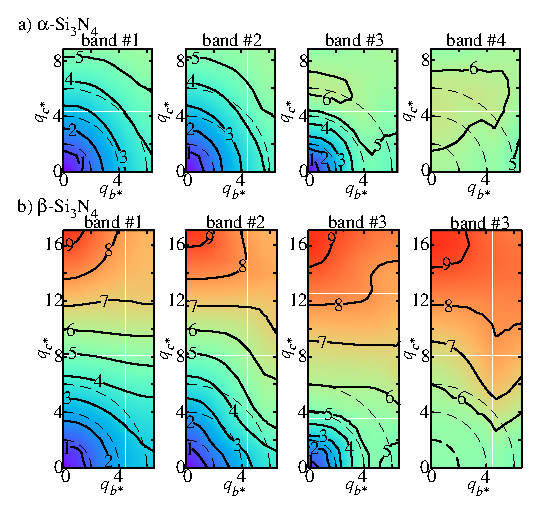
\includegraphics[width=\linewidth]{Fig2_small.eps} \caption{(color
  online) Contour maps of phonon frequency (THz) on the $b^*c^*$
  planes of Brillouin-zones. The coordination in the reciprocal plane 
   are in units of $10^{-2}$ \AA$^{-1}$. The maps for the four lowest-frequency
  phonon modes are shown. The frequency landscapes are formed by simply
  connecting the frequencies of the same band indices, assigned by
  ascending order of frequency at the respective $\mathbf {q}$
  points. \label{fig:Fig3_338} }
 \centering
\end{figure}

We investigate the anisotropy in the $\mathbf{v}_{\lambda}$ by using another
geometry, that is, a cross-section of the Brillouin-zone.
Fig.~\ref{fig:Fig3_338} shows counter maps of $\omega_{\lambda}$  on the
$b^*c^*$ plane.  We show the maps for the four lowest-frequency bands, because
they contribute significantly to the $\boldsymbol{\kappa}$. There were
negligible differences between the distributions on the $b^*c^*$ plane and the
other planes containing the $c^*$ axis.  Thus we select the $b^*c^*$ plane as a
representative.  In the $\alpha$ phase, the distributions are nearly isotropic.
The $\mathbf{v}_{\lambda}$ are thus nearly isotropic. In the $\beta$ phase, the
iso-frequency lines in $0.06 \le q_{c^*} \le 0.12$ \AA$^{-1}$ are rather
parallel to the $q_{b^*}$ axis.  The $\mathbf{v}_{\lambda}$ there orient
closely to the $c^*$ axis direction. This confirms the large anisotropy in the
$\mathbf{v}_{\lambda}$ of the acoustic and low-frequency optical phonon branches
in the $\beta$ phase.

\subsection{Frequency-dependences of $\boldsymbol{\kappa}^\text{c}$, $\mathbf{v}$$_\lambda$ and $\Gamma_\lambda$}

\begin{figure*}[ht]
 \begin{center}
  \includegraphics[width=0.9\linewidth]{figure_dos_jdos_kc_m1010_dos_enlarge.eps}
  \caption{(color online) Microscopic phonon properties of three Si$_3$N$_4$
	  phases. DOS (a), Cumulative thermal conductivity $\mathbf{\kappa}^\text{c}$ and its derivative
	  (b), weighted DOS with $v_{\lambda,i}^2$ (c), and linewidth $\Gamma_\lambda$ (d).
  \label{fig:Fig5_338_rev} }
 \end{center}
\end{figure*}

We have investigated in the previous two sections the anisotropy in the
$\mathbf{v}_\lambda$, which can explain the anisotropy in the
$\boldsymbol{\kappa}$. Here we more completely investigate the characteristic
points in the $\boldsymbol{\kappa}$ by using the phonon properties existing in
the closed form of RTA in Eq.~(\ref{eq:kappa}). These properties are taken over
the Brillouin zone, similar to $\boldsymbol{\kappa}$.  In order to investigate
these properties with respect to the phonon modes, we show in
Fig.~\ref{fig:Fig5_338_rev} frequency distributions of these properties: Phonon
densities of states (DOS), $g(\omega)$, shown in Fig.~\ref{fig:Fig5_338_rev}-a
can be viewed as frequency distributions of heat carriers.  In DOS, a
low-frequency main peak is denoted by an arrow. Considering the band diagrams,
this peak is approximately associated with flattening of acoustic phonon
branches near Brillouin zone boundaries.  In Fig.~\ref{fig:Fig5_338_rev}-b,
$\boldsymbol{\kappa}^c$ and their first derivatives are shown in order to find
the phonon mode contribution to the $\boldsymbol{\kappa}$ clearly. In
Fig.~\ref{fig:Fig5_338_rev}-c, we show weighted DOS with the
vector-direct-product of group velocities (WDOS), $\boldsymbol{h}(\omega)$,
\begin{align}
 \label{eq:wdos}
 \boldsymbol{h}(\omega) = \frac{1}{N_\mathbf{q}Z}
 \sum_\lambda
 \mathbf{v}_\lambda \otimes \mathbf{v}_\lambda
 \delta(\omega-\omega_{\lambda}),
\end{align}
where $Z$ is the number of formula units in the unit cell. WDOS shows the
impacts of $\mathbf{v}_\lambda$ and number of heat carriers.  Phonon linewidths
are a remaining important property.  They are shown as scatter plots of
$(\Gamma_\lambda, \omega_\lambda)$ in Fig.~\ref{fig:Fig5_338_rev}-d. 

Among the panels in Fig.~\ref{fig:Fig5_338_rev}, the $\gamma$ phase has its DOS,
WDOS, and $\Gamma_\lambda$ distribution much different from the others,
consistently with the large differences in the crystal structure. Some of the
differences are remarked as follows:

(1) The DOS peak is located at the highest frequency among the three phases.
This is consistent with the band diagram we have examined. In
the lower frequency side of the peak, the $\gamma$ phase has the lowest intensities among
the three phases, indicating the smallest number of heat carriers. 

(2) In WDOS, for most of the frequencies with phonon modes largely contributing
to $\boldsymbol{\kappa}$, the $h_{xx}$ of the $\gamma$ phase has the next
largest intensities to the $h_{zz}$ of the $\beta$ phase. 

(3) In the $(\Gamma_\lambda,\omega_\lambda)$ plots, for $\omega_\lambda \lesssim
10$
THz, the $\gamma$ phase has approximately twice larger $\Gamma_\lambda$ than the
other phases. 
For this point, we will examine the
$|\Phi_{\lambda\lambda'\lambda''}|^2$ included in Eq.~(\ref{eq:linewidth}),
later. 

Summarizing these remarks, for the $\gamma$ phase, in spite of the large
$\rm{v}_\lambda$ of the phonon modes in the acoustic phonon branches, the large
linewidths and small DOS make the $\kappa^c_{xx}$  not so large and similar to
the $\kappa^c_{xx}$ of the $\beta$ phase.

Next, we compare the properties between the $\alpha$ and $\beta$ phases.  It is
interesting that $\boldsymbol{\kappa}^c$ in the $\beta$ phase still increase
significantly in the higher frequency side to the DOS peak. In this frequency
range, WDOS of the $\beta$ phase show larger intensities than those of the
$\alpha$ phase, while the left two properties (linewidths and DOS) are similar
between the phases. Thus the large $\rm{v}_\lambda$ simply makes the
$\boldsymbol{\kappa}^c$ large there. The large $\rm{v}_\lambda$ in this
frequency range are consistent with the band diagram we have examined. In
Figs.~\ref{fig:Fig5_338_rev}-b and c, the profiles of
$\frac{d\boldsymbol{\kappa}^c_{ii}}{d\omega_\lambda}$ are qualitatively
explained by the $h_{ii}$ with the same indices.  Again, considering the similar
DOS and $\Gamma_{\lambda}$, the different anisotropy in the $\mathbf{v}_\lambda$
simply accounts for the different anisotropy in $\boldsymbol{\kappa}$. 

It is left curious that $\Gamma_\lambda$ are similar between these two phases
although $\mathbf{v}_\lambda$ show marked differences.  We investigate this
further. As for not linewidths but thermal conductivities, Lindsay {\it et
al.}~\cite{Lindsay} found that the experimental thermal conductivities were
inversely proportional to the number of configurations for three phonons
$\{\lambda, \lambda', \lambda''\}$ involved in the three-phonon scattering,
which was referred as the phase space available for the three-phonon
scattering~\cite{Lindsay}.  In analogy to Lindsay {\it et al.}, we can say that
the present linewidth depends on the number of configurations for the available
two phonons, $\{\lambda', \lambda''\}$.  Moreover, it depends on
$|\Phi_{\lambda\lambda'\lambda''}|^2$ as well. We examine these terms
one-by-one. A distribution of two-phonon configurations is represented as a
joint density of states (JDOS),
${D_2(\mathbf{q},\omega)}$,  
\begin{align}
 \label{eq:jdos}
 &D_2(\mathbf{q},\omega) = D_2^{(1)}(\mathbf{q},\omega) +  D_2^{(2)}(\mathbf{q},\omega)
\end{align}
where 
\begin{eqnarray*}
	D_2^{(1)} & = & \frac{1}{N} \sum_{\lambda'\lambda''}\Delta(-\mathbf{q} + \mathbf{q'} + \mathbf{q''}) \nonumber \\
								   & \times & [\delta(\omega + \omega_{\lambda'} - \omega_{\lambda''}) + \delta(\omega - \omega_{\lambda'} + \omega_{\lambda''})],\\
	D_2^{(2)} & = & \frac{1}{N} \sum_{\lambda'\lambda''}\Delta(-\mathbf{q} + \mathbf{q'} + \mathbf{q''}) \nonumber \\
								   & \times & \delta(\omega - \omega_{\lambda'} - \omega_{\lambda''}),
\end{eqnarray*}
with $\Delta$($\mathbf{x}$) giving 1 if $\mathbf{x}$ is a reciprocal lattice
vector and otherwise zero.  In more rigorous study, JDOS should be weighted with
the Bose-Einstein distribution terms appeared in Eq.~(\ref{eq:linewidth}).  We
firstly employ the JDOS to intuitively examine the similarity between the
$\Gamma_{\lambda}$ of the $\alpha$ and $\beta$ phases. The weighted JDOS (WJDOS)
will be briefly shown later including that of the $\gamma$ phase. 

Fig.~\ref{fig:Fig6_338} shows frequency-functions of JDOS at several different
$\mathbf{q}$-points. They have very weak
$\mathbf{q}$-point dependences. At the low frequency region with the phonon modes
largely contributing to the $\boldsymbol{\kappa}$, among the two terms of
$D_2^{(1)}$ and $D_2^{(2)}$ in Eq.~(\ref{eq:jdos}), dominant is $D_2^{(1)}$.
The $D_2^{(1)}$ basically corresponds to the half part ($\omega \geq  0$) of the
auto-correlation function of the DOS. The DOS for both of the $\alpha$ and
$\beta$ phases in Fig.~\ref{fig:Fig5_338_rev}-a have a frequency gap. The
$D_2^{(1)}$ reflect this DOS feature, dropping suddenly around 0 THz and showing
a small shoulder around 5 THz, which corresponds to the width of the gap.
Moreover the $D_2^{(1)}$ shows a broad peak around 18 THz, which corresponds to
the frequency giving the largest correlation between the DOS in the
higher and lower frequency portions to the gap.  Because the gap is originated
from the differences in the vibrations of the planer NSi$_3$ contained in both
of the $\alpha$ and $\beta$ crystal structures,~\cite{kuwabara} the major shapes
of the $D_2^{(1)}$ are similar in these phases.
In the present Si$_3$N$_4$ system, the number of phonon modes in the acoustic
and low-frequency optical phonon branches are much smaller than 
the number of the other phonon modes. 
Therefore JDOS are mainly determined by the other phonon modes, even if the
frequency is close to the $\omega_\lambda$ of the acoustic and low-frequency
optical phonon modes.

\begin{figure}[ht]
 \centering
  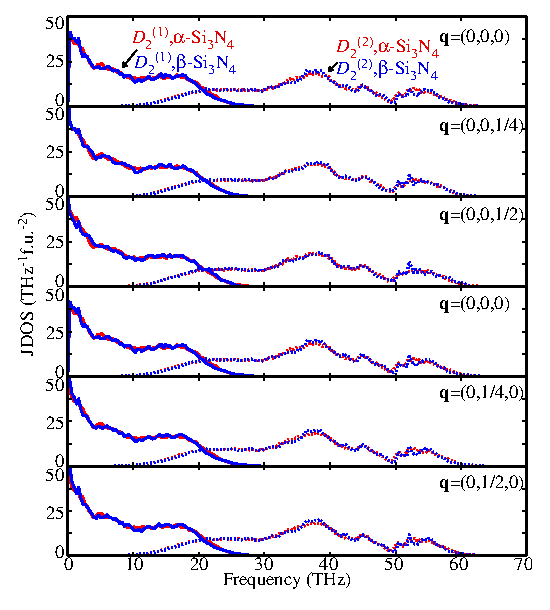
\includegraphics[width=0.9\linewidth]{figure_jdoss.eps} \caption{(color
	  online) JDOS of $\alpha$- and $\beta$-Si$_3$N$_4$ at different $\mathbf q$ points.
  The first and forth rows are JDOS at the same $\Gamma$-point but calculated
  with the polarization for non-analytic term correction set along $c^*$ and
  $b^*$, respectively. \label{fig:Fig6_338} }
 \centering
\end{figure}

The WJDOS of $N_2(\omega,\mathbf{q})$ are shown in Fig.~\ref{fig:Fig_wjdos}. For
the comparison among the three phases, we only show the frequency distributions
at $\mathbf{q}=(0,0,0)$. Similar to JDOS, the $\mathbf{q}$ dependences of the
WJDOS were negligible. The terms of the two classes corresponding to $D_2^{(1)}$
and $D_2^{(2)}$ in JDOS are denoted as $N_2^{(1)}$ and $N_2^{(2)}$.  The
weighting factors reduce the $N_2^{(1)}$ near 0 THz and enhance the $N_2^{(2)}$
in the high frequency range. However the $N_2^{(1)}$ are dominant in the low
frequency range where the phonon modes largely contribute to the
$\boldsymbol{\kappa}$. These $N_2^{(1)}$ have similar intensities there, having
insignificant differences for the impacts on the linewidths among the three
phases. 

\begin{figure}[ht]
 \centering
  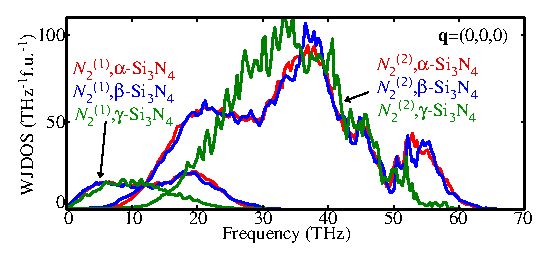
\includegraphics[width=0.9\linewidth]{Fig_wjdos.eps} \caption{(color
	  online) Comparison of WJDOS at $\mathbf{q}=(0,0,0)$ for 300 K among the three phases. 
		  } \label{fig:Fig_wjdos} 
 \centering
\end{figure}

\begin{table}[ht]
	\caption{\label{table:aveavepp} Averages of
	$\Phi_{\lambda\lambda'\lambda''}$ over frequency ranges of
	$\omega_\lambda$ (0--15 and 0--35 THz) and all ($\lambda'$,$\lambda'$). The
	values are in units of 10$^{-10}$ eV$^2$f.u.$^{-1}$.}
 \begin{ruledtabular}
  \begin{tabular}{cccc}
	  \multirow{2}{*}{Frequency Range (THz)}
   & \multicolumn{3}{c}{Phase}  \\
   \cline{2-4}
   & $\alpha$ & $\beta$ & $\gamma$ \\
   \hline
   \multirow{1}{*}{0--15}
   & 2.66  &  2.63  & 5.76 &    
   \multirow{1}{*}{0--30}
   & 13.1 & 13.0 & 11.4 &     
  \end{tabular}
 \end{ruledtabular}
\end{table}

As for $|\Phi_{\lambda\lambda'\lambda''}|^2$, in Table.~\ref{table:aveavepp},
they are averaged over two kinds of frequency ranges of 0--15 or 0--30 THz for
$\omega_\lambda$ and all indices in $\lambda'$ and $\lambda''$.  The averages
are similar between the $\alpha$ and $\beta$ phases. With these similar impacts
of the (W)JDOS and $|\Phi_{\lambda\lambda'\lambda''}|^2$, the linewidth
distributions in Fig.~\ref{fig:Fig5_338_rev}-d of the two phases are similar.
For the $\gamma$ phase, the large $|\Phi_{\lambda\lambda'\lambda''}|^2$ in the
lower frequency range attribute to the large linewidths.  We set the two
frequency ranges for $\omega_\lambda$ in accordance with the lower frequency
range covering the phonon modes significantly contributed to the
$\boldsymbol{\kappa}$. For any of such two frequency ranges, the qualitative
characters of the averages were confirmed as invariant.  

Finally, a small but interesting difference in linewidth distributions are seen
between the $\alpha$ and $\beta$ phases in Fig.~\ref{fig:Fig5_338_rev}-d.
$\Gamma_\lambda$ below 5 THz are aligned on a single smooth line in the $\alpha$
phase, while those in the $\beta$ phase are scattered roughly on two branches.
This difference is investigated with directions of the atomic vibrations of the
phonon modes. Fig.~\ref{fig:Fig7_338} enlarges the
$(\Gamma_\lambda,\omega_\lambda)$ plots in this frequency range. In
Fig.~\ref{fig:Fig7_338}-a, the $\Gamma_\lambda$ are classified using colors
according to the sums of the squares of the eigenvector components along the
$\mathbf{q}$; the sum is 1 for a perfectly longitudinal wave. However, these
sums have no clear color-contrast distinguishing the two branches in the $\beta$
phase.  Fig.~\ref{fig:Fig7_338}-b shows the same plot as
Fig.~\ref{fig:Fig7_338}-a, but with colors according to the sums of the squares
of the eigenvector components along the $ab$ plane, which has 1 when the
eigenvectors lie on the $ab$ plane. There is a tendency in the $\beta$ phase
that  $\Gamma_\lambda$ are large for vibrations along the $ab$ plane.
Therefore, within the single-mode RTA, for the phonon modes below 5 THz, all of
which belong to the acoustic phonon branches, vibration modes along the $ab$
plane are more easily scattered in the $\beta$ phase, no matter whether they are
longitudinal or transverse. For the panel of $\beta$-Si$_3$N$_4$ in
Fig.~\ref{fig:Fig7_338}-b, a straight line splits the phonon modes to two
groups. The numbers of the phonon modes assigned to the larger and smaller
$\Gamma_\lambda$ groups are 157 and 58, whose ratio is consistent to the
population ratio of the vibration modes along and out of the $ab$ plane.

\begin{figure}[ht]
 \centering
  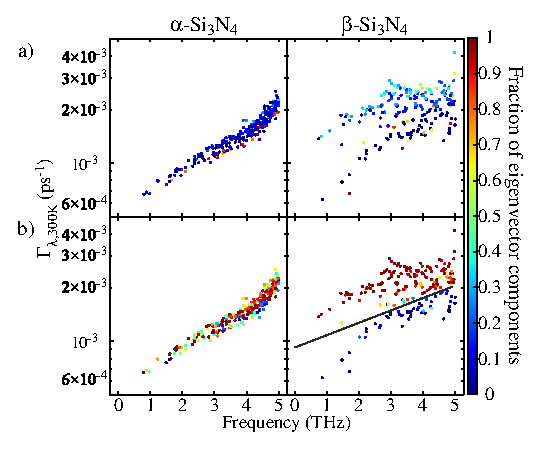
\includegraphics[width=\linewidth]{figure_analyze_gamma3_m1010_print.eps} \caption{(color
	  online) Distribution of linewidths $\omega_\lambda$ $\leq$ 5 THz
		  with colors with respect to strengths of eigenvector components along $\mathbf q$ (a)
		  and on $ab$ plane (b).} \label{fig:Fig7_338} 
 \centering
\end{figure}

\section{Summary}

In the present study, we investigate the lattice thermal conductivities of the
three Si$_3$N$_4$ phases, by using the lattice dynamics based on the first
principles interatomic force constants. The main remarks are as follows:

1) In the $\alpha$- and $\beta$-Si$_3$N$_4$, whose crystal structures are
characterized by the stacking manners of the basal layer structures, which
largely alter $\boldsymbol{\kappa}$. The $\boldsymbol{\kappa}$ of
$\alpha$-Si$_3$N$_4$ is rather isotropic, while the $\kappa$$_{zz}$ of the
$\beta$ phase is twice or more larger than the other $\kappa_{ii}$ of the three
phases.

2) In the $\alpha$ phase, the acoustic mode phonons below 6 THz are the main
heat carriers, while in the $\beta$ phase, the phonons below 12 THz contribute
to the $\boldsymbol{\kappa}$. The group velocities alone qualitatively explain
this and the different behaviours in $\boldsymbol{\kappa}$ between these phases.
This is partly because JDOS is insensitive to the group velocities of the phonon
modes whose fraction is small.

3) In the $\gamma$ phase, the $\kappa_{xx}$ is relatively small. The
$\kappa^c_{xx}$ is similar to that of $\beta$-Si$_3$N$_4$. Its large
$|\Phi_{\lambda\lambda'\lambda''}|^2$
and small DOS attribute to these characters.

\section*{ACKNOWLEDGMENTS}
The present work was partly supported by Grants-in-Aid for Scientific
Research of MEXT, Japan (Grant No. 15K14108 and ESISM (Elements Strategy
Initiative for Structural Materials) of Kyoto University).

\appendix
\section{Pressure dependence of lattice thermal conductivity of $\gamma$-phase}
\begin{figure}[ht]
 \begin{center}
  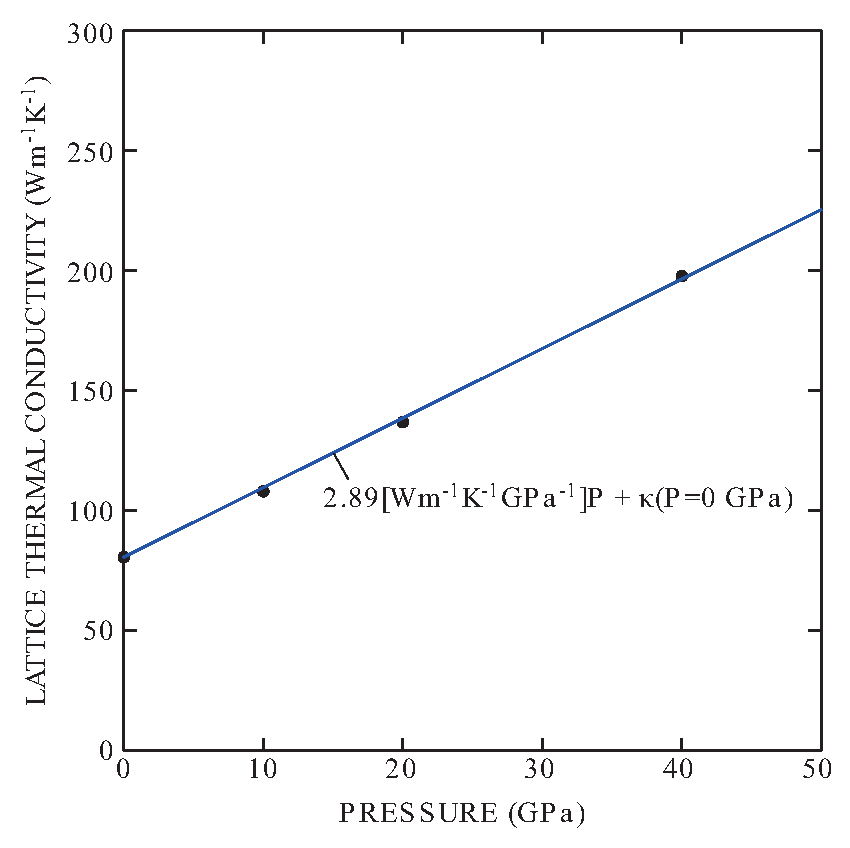
\includegraphics[width=0.80\linewidth]{S1.eps} \caption{(color online)
  Pressure dependence of lattice thermal conductivity of $\gamma$-Si$_3$N$_4$.  \label{fig:S1} }
 \end{center}
\end{figure}
\bibliography{Si3N4}
\end{document}
